\chapter{Calculation of the Formation Energy of the [$Cu_{Zn}^- + Zn_{Cu}^+$] Defect Pair in {\CZTS}}\label{Cu-Zn_defects_calc}

* Add details of DFT supercell calc here + need for hybrid-DFT for defects (see Lany paper) + how full formation eqn simplifies for charge neutral defect + equilibrium Cu-Zn defect conc and need for MC because not dilute (see MRes 1 and add plot to appendix?)

\begin{itemize}
\item General defect formation E eqn
\item Simplified version for charge neutral defect complex
\item Brief overview of DFT and need for hybrid-DFT for defect calculations
\item The supercell method for defect calculations
\item General proceedure: ENCUT, kpoints, geom opt and one-shot
\item Jonathan's conv test spreadsheet?
\item Visual of supercell defect
\item Expected concentration greater than dilute limit + need for MC + plot of conc?
\end{itemize}


\begin{figure}[h!]
  \centering
    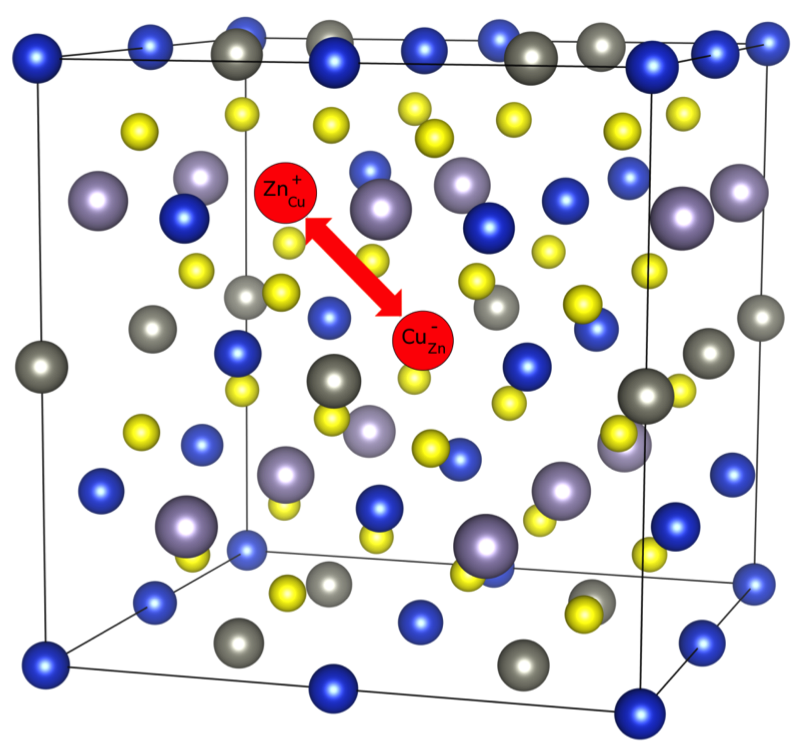
\includegraphics[width=0.6\textwidth]{figures/Cu-Zn_defect.png}
    \caption{64 atom supercell of {\CZTS} showing a substitution of Cu and Zn ions that results in the formation of the nearest neighbour antisite defect pair.}
  \label{Cu-Zn_defect}
\end{figure}



When defect concentrations are less than 1\%, it is usually assumed that the system is in the dilute defect limit where defects can be considered to be non-interacting. Using statistical thermodynamics for point defects, an expression for the equilibrium concentration of point defects as a function of temperature can be obtained \cite{thermodynamics}. This is shown in equation \ref{defect_conc}, where N is the number of sites, $E_f$ is the defect formation energy, $k_B$ is the Boltzmann constant and T is the temperature of the system.
\begin{equation} \label{defect_conc}
n = Ne^{\frac{-E_f}{k_BT}}
\end{equation}
The probability of defect formation as a function of temperature is given by the exponential expression in equation \ref{defect_conc}. Defect formation energies from the DFT calculations were halved to take an average of the formation energy per defect during the formation of an antisite pair before being inserted into this expression. This is plotted against temperature in figure \ref{dilute_defects}. \\

It can be seen from figure \ref{dilute_defects} that the probability of defect formation at a typical annealing temperature of 550K \cite{anneal_temp} is approximately 3-4\%.
From data in table \ref{defect_formation_energies}, the distance between the defects decreases slightly during the geometry optimisation from that of the undefected system.
The point defects (the $Cu_{Zn}$ and $Zn_{Cu}$ antisites) form the defect complex [$Cu_{Zn}^- + Zn_{Cu}^+$]. The point defects become associated with one another due to a Coulomb interaction between the effective +1 and -1 charge that results from substituting species with a +1 charge with a species with a +2 charge and vice versa. The high equilibrium concentrations of antisite defects predicted suggests that it is not sufficient to consider the $Cu_{Zn}$ and $Zn_{Cu}$ antisites as non-interacting point defects and that we must instead consider a system of interacting defects.


\begin{figure}[h!]
  \centering
    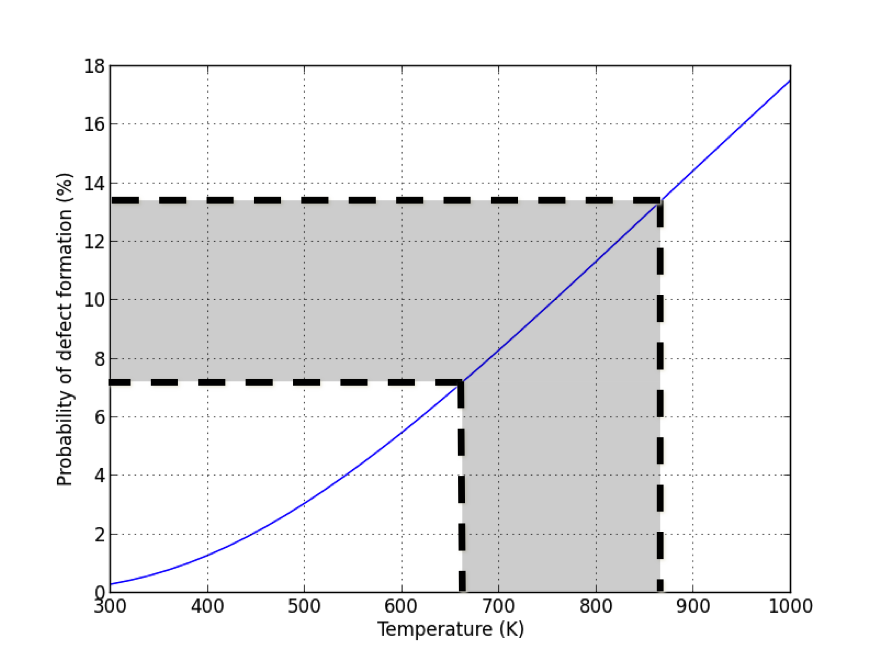
\includegraphics[width=0.9\textwidth]{figures/Cu-Zn_eqm_conc.png}
    \caption{Probability of nearest neighbour [$Cu_{Zn}^- + Zn_{Cu}^+$] defect formation as a function of temperature based on the equilibrium defect concentration from classical thermodynamics. The shaded region indicates typical annealing temperatures used in the synthesis of {\CZTS}.}
  \label{Cu-Zn_eqm_conc}
\end{figure}
